\chapter{Introduction}
\label{ch:Introduction}
This chapter introduces the bacholor thesis's problem and derived objective.

\section{Initial Situation \& Problem}
\label{sec:InitialSituation}
In 1970, Eugene Fama introduced the \gls{emh}, which argues that publicly available information does not allow investors to consistently outperform a global benchmark such as the S\&P500 \citep{fama1970efficient}. In 1988, Halbert White attempted to find empirical evidence against the \gls{emh} by using an \gls{ann} to predict IBM's daily stock returns. He was unable to find convincing statistical evidence against it \citep{white1988economic}, thereby supporting Fama's hypothesis.
\newline
\newline
Undeterred, major financial institutions such as Bloomberg have devoted significant resources to achieving alpha, which essentially means outperforming the market. Machine learning plays a pivotal role in this endeavour, encompassing tasks such as sentiment analysis and named entity recognition \citep{wu2023bloomberggpt}.
\newline
\newline
Alongside these established institutions, new entrants have joined the hunt for alpha. Neo-brokers such as Robinhood have democratised financial services and as a result have seen significant user growth in recent years, as shown in figure \ref{fig:users_RH}. However, it's worth noting that the average Robinhood trader has failed to outperform the S\&P 500 index \citep{canellis-2020}, in line with the \gls{emh}.

\begin{figure}[ht]
    \centering
    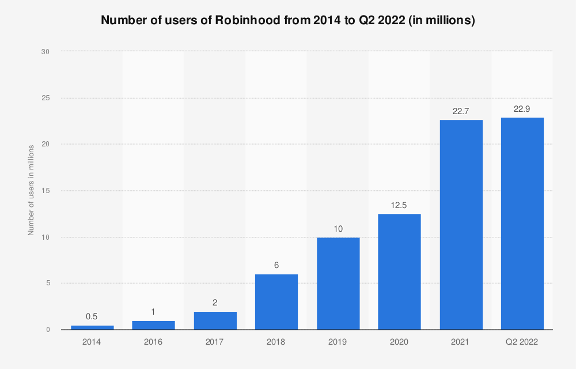
\includegraphics[width=0.85\textwidth]{./assets/img/users_rh.png}
    \caption{Figure shows the number of users on Robinhood from 2014 to Q1 2022. Figure from \cite{statista_robinhood}.}
    \label{fig:users_RH}
\end{figure}

\clearpage
\noindent
This raises a fascinating question: If researchers like White cannot find empirical evidence against the \gls{emh}, and the average Robinhood trader is also not able to beat a global benchmark like the S\&P500, why are financial institutions still trying to achieve alpha by processing financial data with machine learning models?

\section{Research Objective}
\label{sec:ResearchObjective}
This empirical research project aims to train several machine learning models on historical cryptocurrency price and volume data, and evaluate their performance against well-known momentum indicators as baselines and a global benchmark.